\chapter{Time is represented in the neural activity}
\label{chap:time_is_represented}

Here we measured whether there is a representation for time in neural activity, based on single-unit recordings on rats' Pre Frontal Cortex. For such, we compared decoding performance in the original data versus in bootstrapped data, which is created by shuffling the time bins of the original data in each trial. The fundamental distinction between shuffled data and the original is that the temporal order has been disrupted. If decoding performance on shuffled data is equal to the original, then we can infer that the temporal ordering of activity is not essential for decoding, and consequently it is not time that is being decoded. Alternatively, if decoding performance is significantly better in the original activity, then time-ordering is driving decoding performance. 

The neural population activity is averaged in bins of 100ms each, from the nosepoke onset (0 - 100 ms) until 1500ms, for a total of 15 population activity vectors per trial. Each bin is tagged with its starting time. In classification the tag is treated as a label, and the problem is treated as multiclass classification: each population vector is classified as one of the 15 possible labels (0, 100, 200, ..., 1400). Alternatively, in regression the tag is treated as a continuous variable, and population vectors are mapped to real values, that can be intermediate values between the bins (e.g. 150). Moreover, in both cases we measure the performance using the explained variance (see \ref{sub:expvar})

\section{We can predict elapsed time using the instantaneous firing rate}
    \begin{figure}
        \centering
        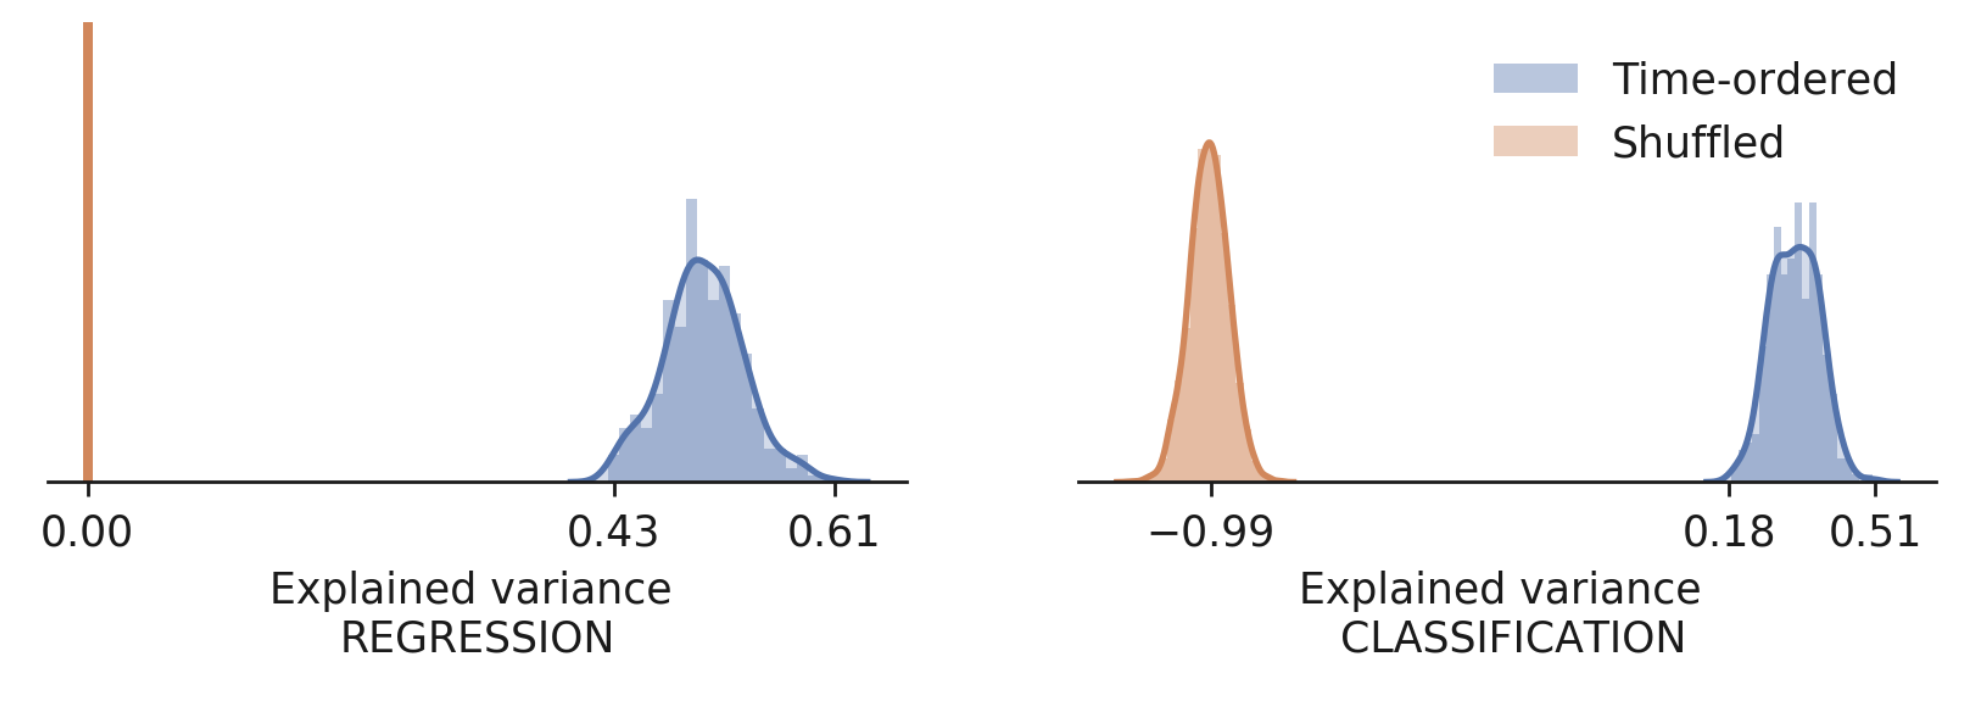
\includegraphics[width=\textwidth]{figures/bootstrap_distribution.png}
        \caption[Comparison between classifier predictions for time-ordered versus time-shuffled population activity]{Comparison between classifier predictions for time-ordered versus time-shuffled population activity. The figure shows the distribution of decoding performances for two decoding methods, in each case comparing with performance in the time-shuffled activity. Either using classification or regression, the population activity differs considerably from the bootstrap, having no overlap.}
        \label{fig:bootstrap_distribution}
    \end{figure}
    
    In figure \ref{fig:bootstrap_distribution} we compare the distribution of decoding performance between shuffled and time-ordered population activities. The distributions are completely separated, giving a p-value of approximately 0 (T-values 974 and 486 for regression and classification) in a t-test. The divergence from bootstrapped data is robust to whether we use regression or classification, as in both cases the distributions have no overlap. The choice of metric also does not change results, in the cases of Pearson's r and accuracy (not shown). 
    
    \begin{figure}[ht]
        \centering
        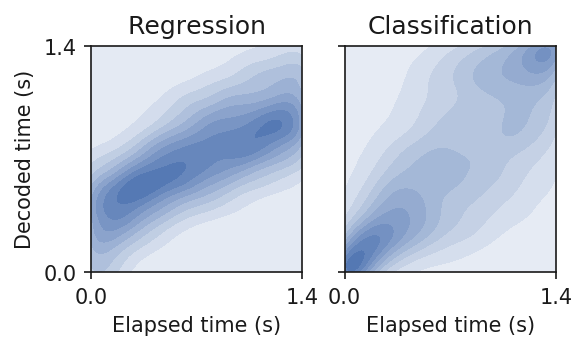
\includegraphics{figures/clf_reg_kde_simple.png}
        \caption[Distribution of predictions show structure]{Distribution of predictions show structure. Figures show two types of algorithm used to assess activity - regression and classification. Darker blues indicate higher density of points. For a given elapsed time, the vertical upon it is the distribution of all predictions calculated over neural activity extracted at that time.}
        \label{fig:decoding_kde_boot}
    \end{figure}
    
    To further assess our decoding results, we look into the distribution of predictions according to the elapsed time of the activity. To this end, we follow a k-fold cross-prediction approach: we separate the trials into 20 groups, or \textit{folds}, evaluating predictions for each fold after training in the 19 other folds. The folds are approximately the same size, with each trial giving rise to 15 predictions, one for each bin of population activity.
    
    We can see the full distribution by kernel-density-estimation in figure \ref{fig:decoding_kde_boot}, and a simpler version with mean and variance in figure \ref{fig:decoding_line_boot}. We can see in \ref{fig:decoding_line_boot} that the mean prediction has a positive inclination, showing that activity from later in the trial is predicted in average with higher values. While this is seen both in classification and regression, they have distinct patterns of errors, showed in \ref{fig:decoding_kde_boot}, with regression tending towards the mean values while classification tends towards the borders. Anyhow, the positive inclination is indicative of the presence of information in the neural activity, and is consistent with the positive evaluation of metrics shown in \ref{fig:bootstrap_distribution}.
    
    \begin{figure}[ht]
        \centering
        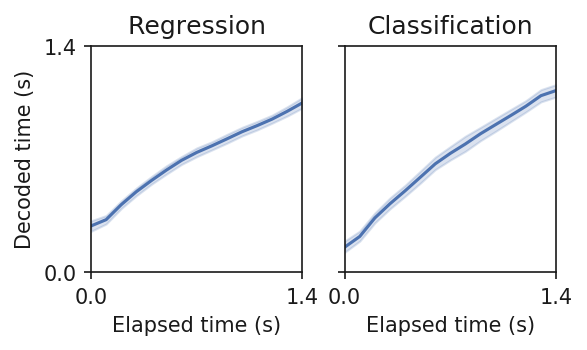
\includegraphics{figures/clf_reg_mean_simple.png}
        \caption[Summary of prediction distributions have positive inclination]{Summary of prediction distributions have positive inclination. Figures show two types of algorithm used to assess activity - regression and classification. The darker line is the average decoded value for all data points extracted from a given Elapsed Time. The bands represent the standard deviation around that average. Since the distributions are not necessarily gaussian, as can be seen in figure \ref{fig:decoding_kde_boot}, the mean and standard deviation are not a full description. Nevertheless, the positive inclination shows there is a tendency to decode bigger times for neural activity coming from bigger elapsed times in the trial.}
        \label{fig:decoding_line_boot}
    \end{figure}

% \section{There is time-warping consistent with timing behavior}
